\providecommand{\main}{../../../..}
\documentclass[\main/dresen_thesis.tex]{subfiles}
\begin{document}
  \label{sec:doubleLayers:vsm}

  \begin{figure}[tb]
    \centering
    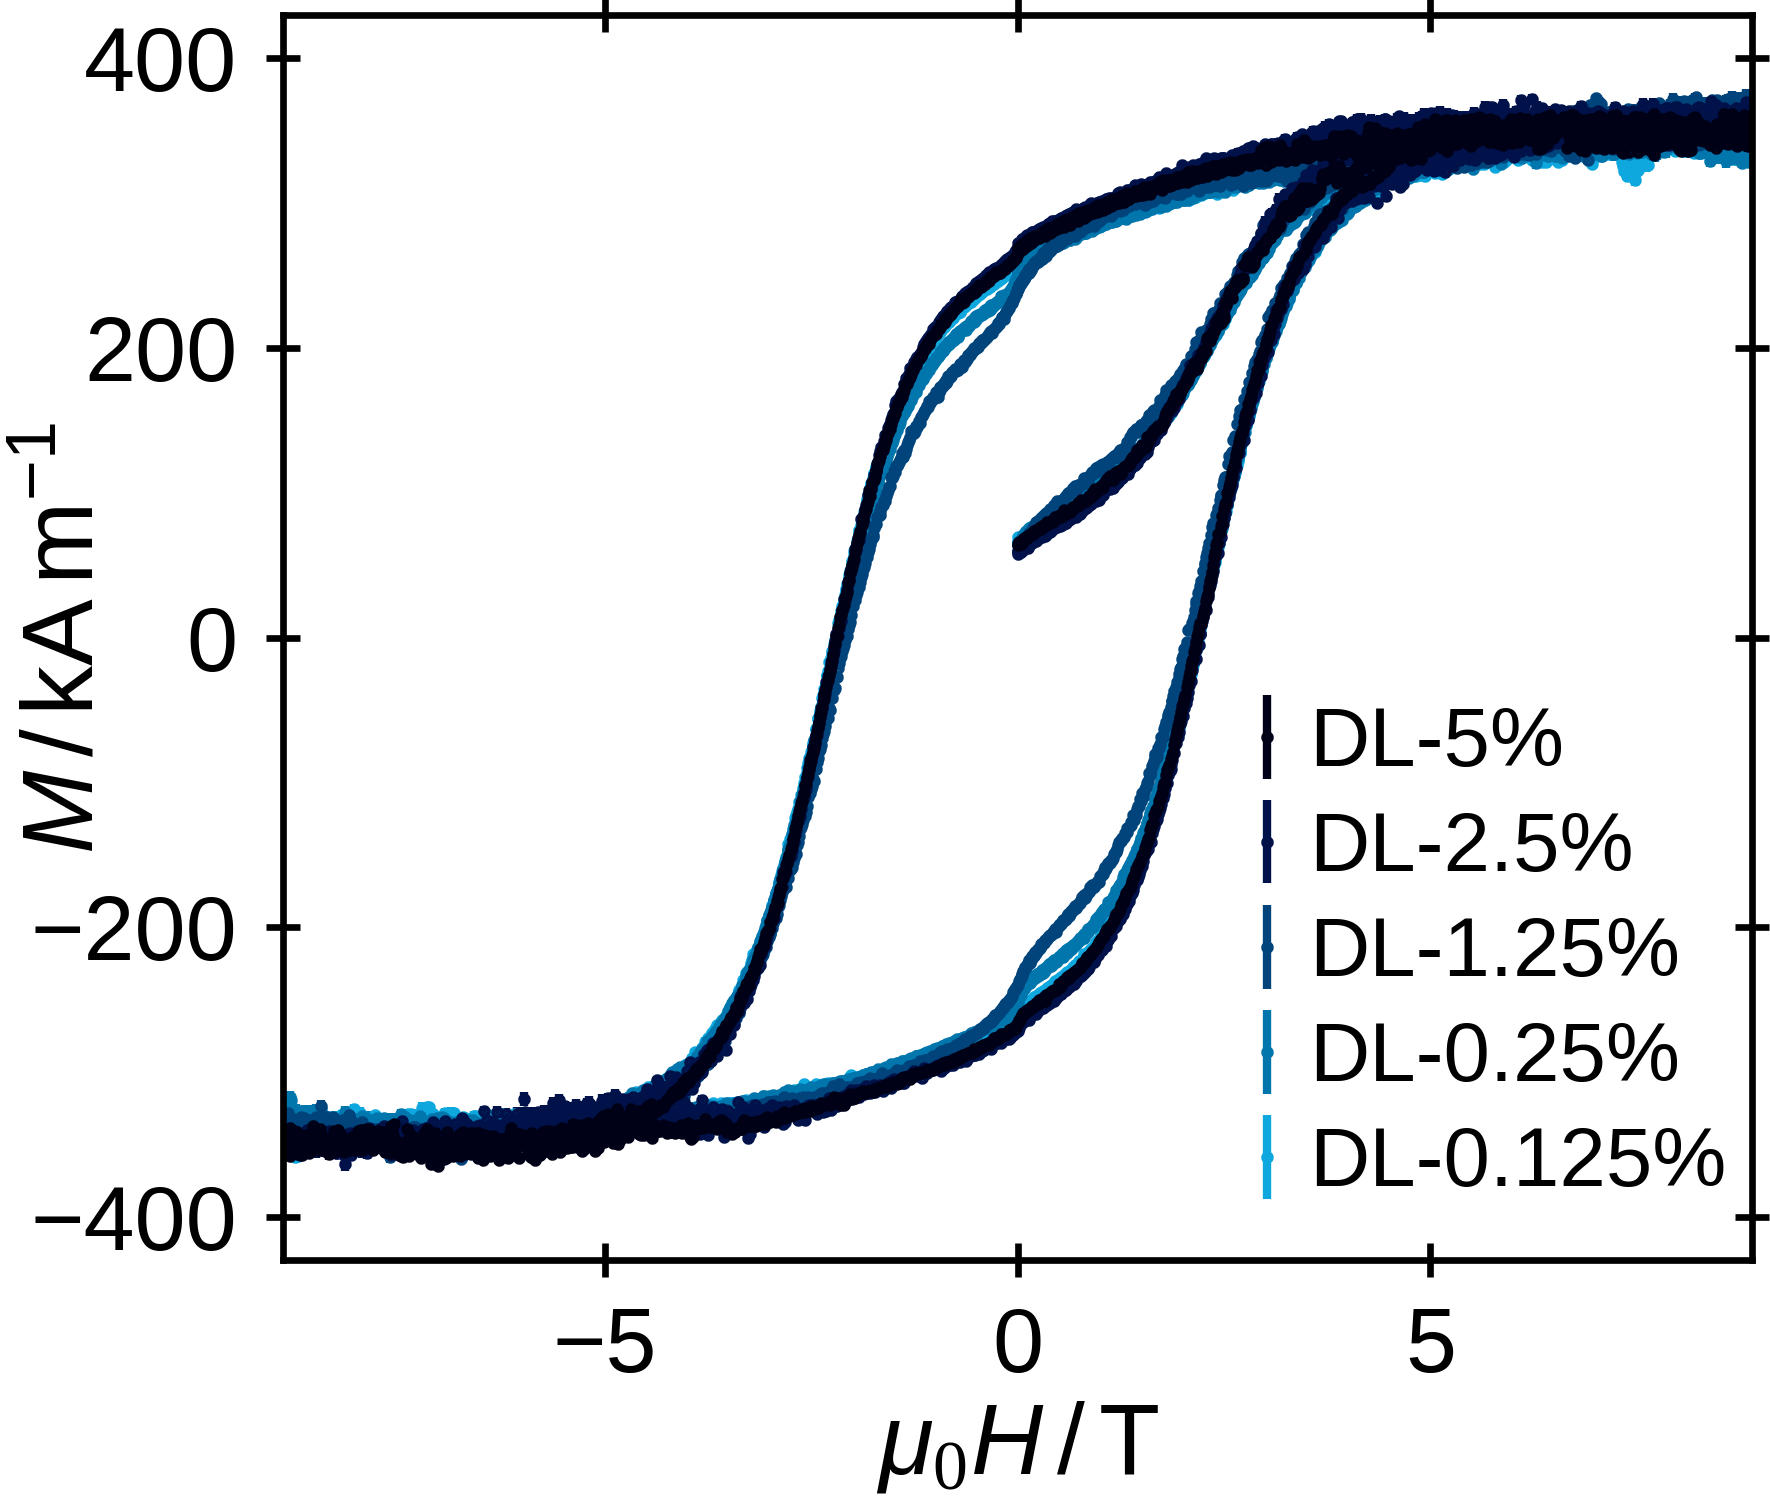
\includegraphics{doublelayers_PPMS_10K_allSamples}
    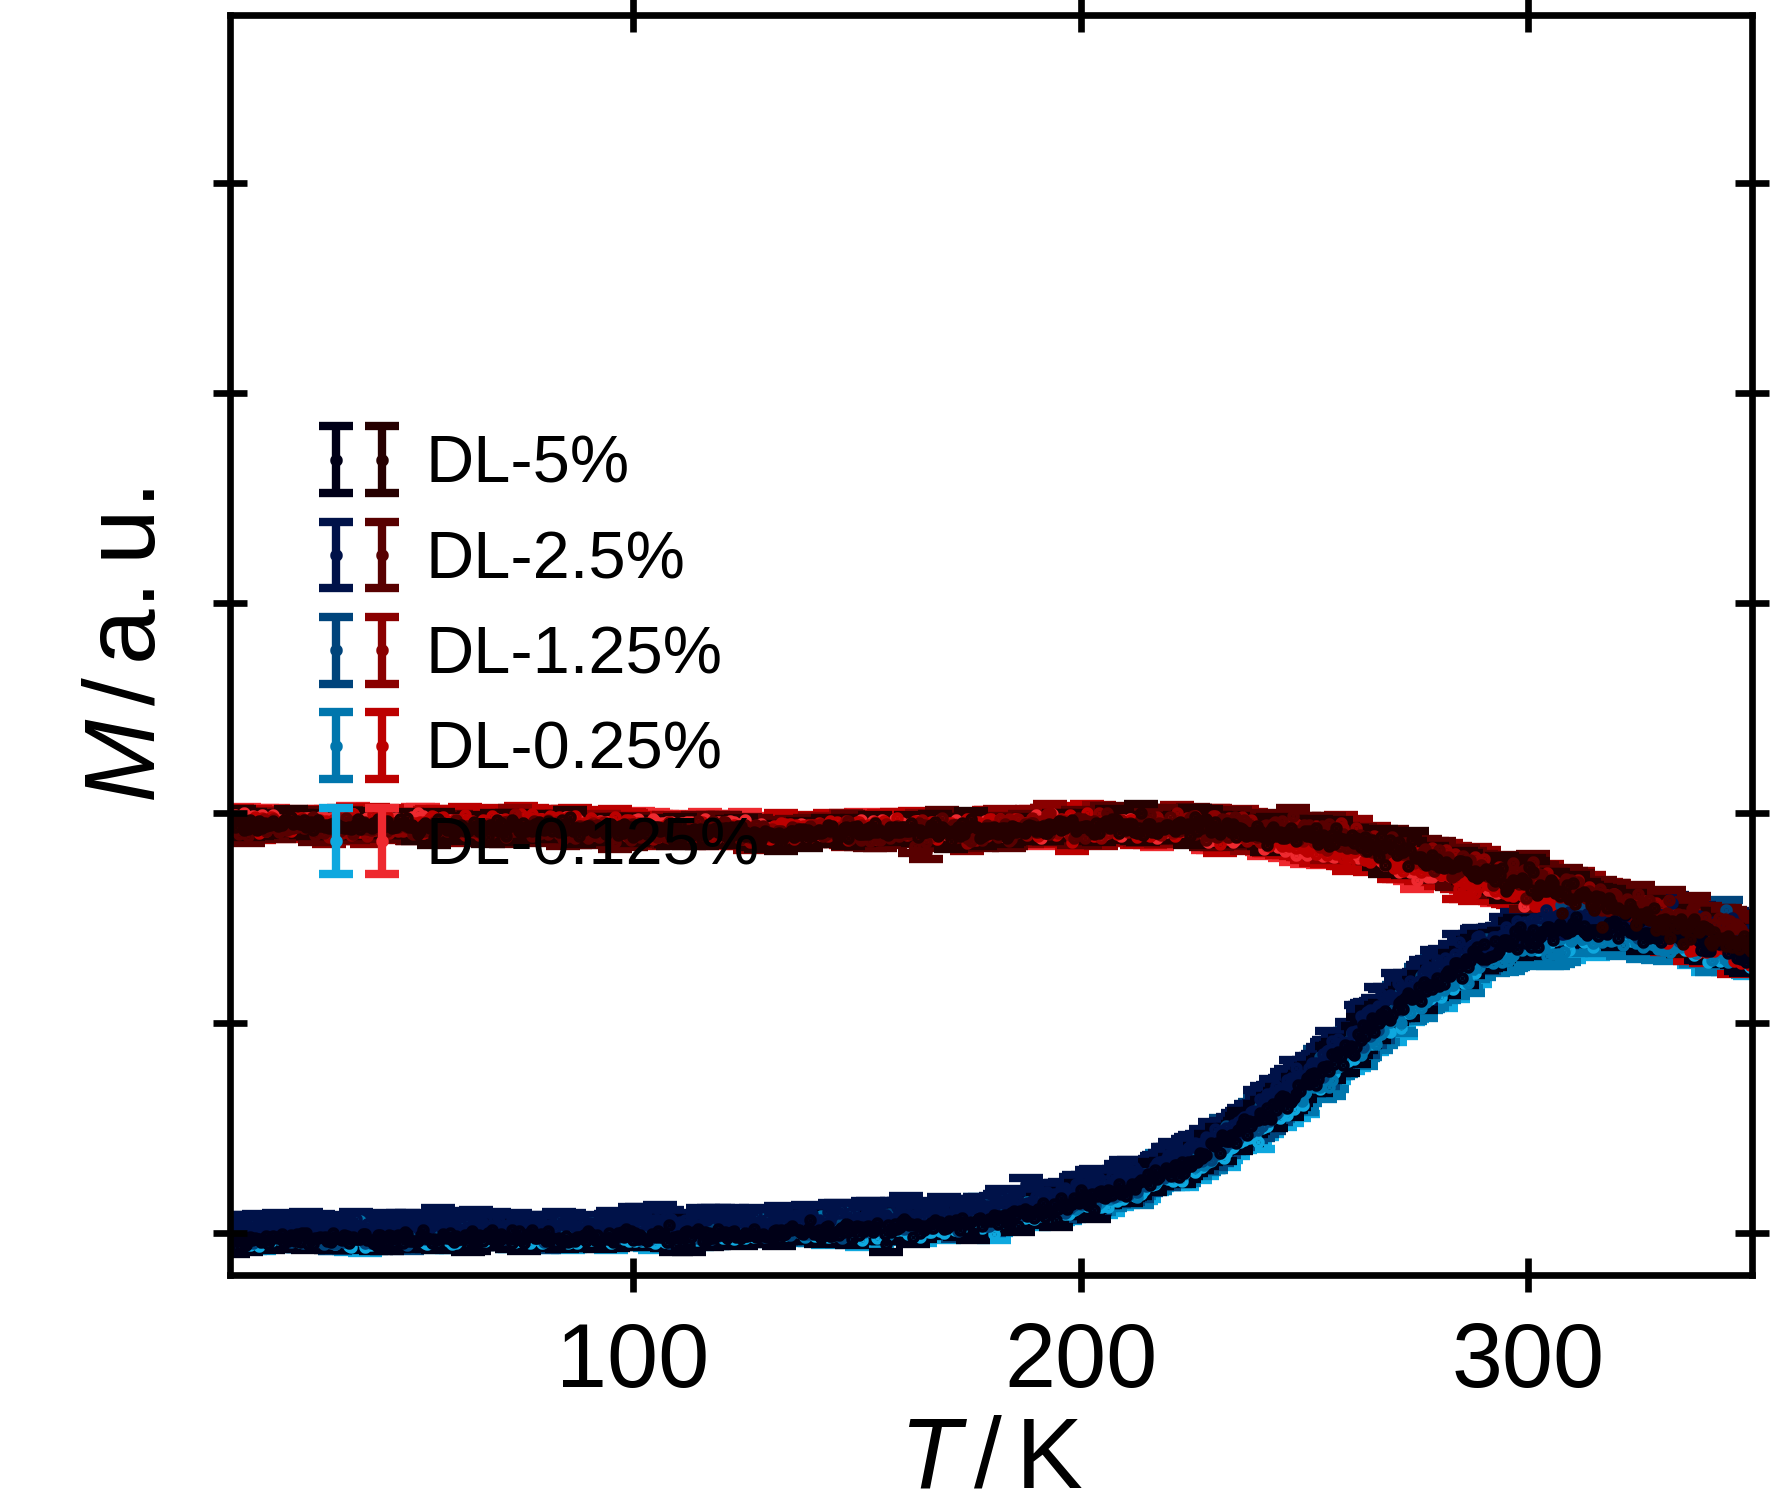
\includegraphics{doublelayers_PPMS_ZFC_FC_allSamples}
    \caption{\label{fig:doubleLayers:zfcFCData}Field- (left) and temperature-dependent (right) magnetization of the double layers. The hysteresis are each measured at a temperature of $10 \unit{K}$ after cooling in zero field, and the temperature-dependent ZFC/FC magnetizations are taken with a field of $10 \unit{mT}$ while warming the sample.  To discuss the qualitative differences, the zero-field cooled and field cooled data, as well as the respective data of the samples with varied spacer thicknesses are shifted by a constant factor.}
  \end{figure}
  Each double layer has been measured field- and temperature-dependent with the same procedure and conditions for direct comparison of the magnetic properties.
  As each double layer sample is prepared from the same dispersion and with a similar procedure, differences in the magnetic properties should be attributable to dipolar interlayer coupling as the PMMA thickness is the only varied parameter.
  In \reffig{fig:doubleLayers:zfcFCData} both are shown for the double layer samples, sorted with respect to the varied PMMA thickness.
  A close inspection of temperature dependent magnetization shows that they all closely resemble each other and no significant difference can be observed across the samples.
  Similar to the monolayer sample in \refsec{sec:monolayers:magneticStructure:vsm}, a blocking temperature around $315 \unit{K}$ is observed as peak temperature in the zero-field cooled magnetization.
  No major shift in that peak position can be observed within the resolution of the measurement, which could otherwise have been a sign for interlayer interaction.

  Subtle differences can however be seen in the hysteresis at $10 \unit{K}$.
  Similar to the monolayer sample, a small jump in the magnetization is visible around $\pm 100 \unit{mT}$.
  The strength is visibly changing from sample to sample, without showing a systematic with respect to the PMMA layer thickness.
  Whereas it appear to be nearly invisible for the lowest PMMA concentration sample DL-0.125\%, it appears clearly visible for DL-0.25\%, reduces in size for DL-1.25\% and becomes stronger again for DL-2.5\%.
  As one would expect from dipolar coupling a reduction of interaction effects with increasing layer thickness and as the jump also appears in monolayer samples, it is probable that this effect is not directly correlated to dipolar interlayer interaction but an uncontrolled property of the nanocube arrays themselves.
  Otherwise the hysteresis resemble each other closely, where each has a coercive field in the magnitude of $2.16(3) \unit{T}$, in agreement with the monolayer sample.
  % In literature, the jump can be found in multiple works discussing cobalt ferrite nanoparticles \cite{Xu_2015_Simul, Fu_2012_Uniqu, Lima_2017_Waspw}.
  % The authors give multiple explainations ranging from dipolar interaction between the particles, to surface spin reorientation, o
  % At the state of this thesis it is yet unclear what the true nature of the jump at low fields is.

  

  % \begin{table}[!htbp]
  %   \centering
  %   \caption{\label{tab:looselyPackedNP:nanoparticle:gisaxs}Parameters for the hard-sphere structure factor in Percus-Yervick approximation shown in for both SC-IOS-11 and SC-IOS-7. $R_\mathrm{HS}$ is the hard-sphere radius and $\eta$ the packing fraction of the structure factor.}
  %   \begin{tabular}{ c | l | l }
  %     \rule{0pt}{2ex} \textbf{GISAXS}  & \textbf{SC-IOS-11} & \textbf{SC-IOS-7} \\
  %     \hline
  %     \rule{0pt}{2ex} $R_\mathrm{HS} \, / \unit{nm}$          & $5.655(2)$           & $3.872(4)$\\
  %     \rule{0pt}{2ex} $\eta          \, / \unit{\%}$          & $43.88(3)$           & $34.20(9)$\\
  %     \hline
  %   \end{tabular}
  % \end{table}
\end{document}